\begin{enumerate}[label=\thesubsection.\arabic*, ref=\thesubsection.\theenumi]
	
	\item Evaluate:
	\begin{align*}
		\lim_{x \to 0} \frac{e^x - 1}{\sqrt{1 - \cos x}}
	\end{align*}
	\hfill \brak{12, 2003}
	
	\solution
	From \eqref{eq:exp_taylor} and \eqref{eq:half_angle_cos}:
	\begin{align}
		\lim_{x \to 0} \frac{1 + x + O\brak{x^2} - 1}{\sqrt{2\sin^2\brak{\frac{x}{2}}}} &= \lim_{x \to 0} \frac{x}{\sqrt{2}\abs{\sin\brak{\frac{x}{2}}}}
	\end{align}
	Evaluating the one-sided limits:
	\begin{align}
		\lim_{x \to 0^+} \frac{x}{\sqrt{2}\sin\brak{\frac{x}{2}}} &= \sqrt{2}, \quad \lim_{x \to 0^-} \frac{x}{-\sqrt{2}\sin\brak{\frac{x}{2}}} = -\sqrt{2}
	\end{align}
	Since the left-hand and right-hand limits are not equal, the limit does not exist.
	\begin{figure}[H]
		\centering
		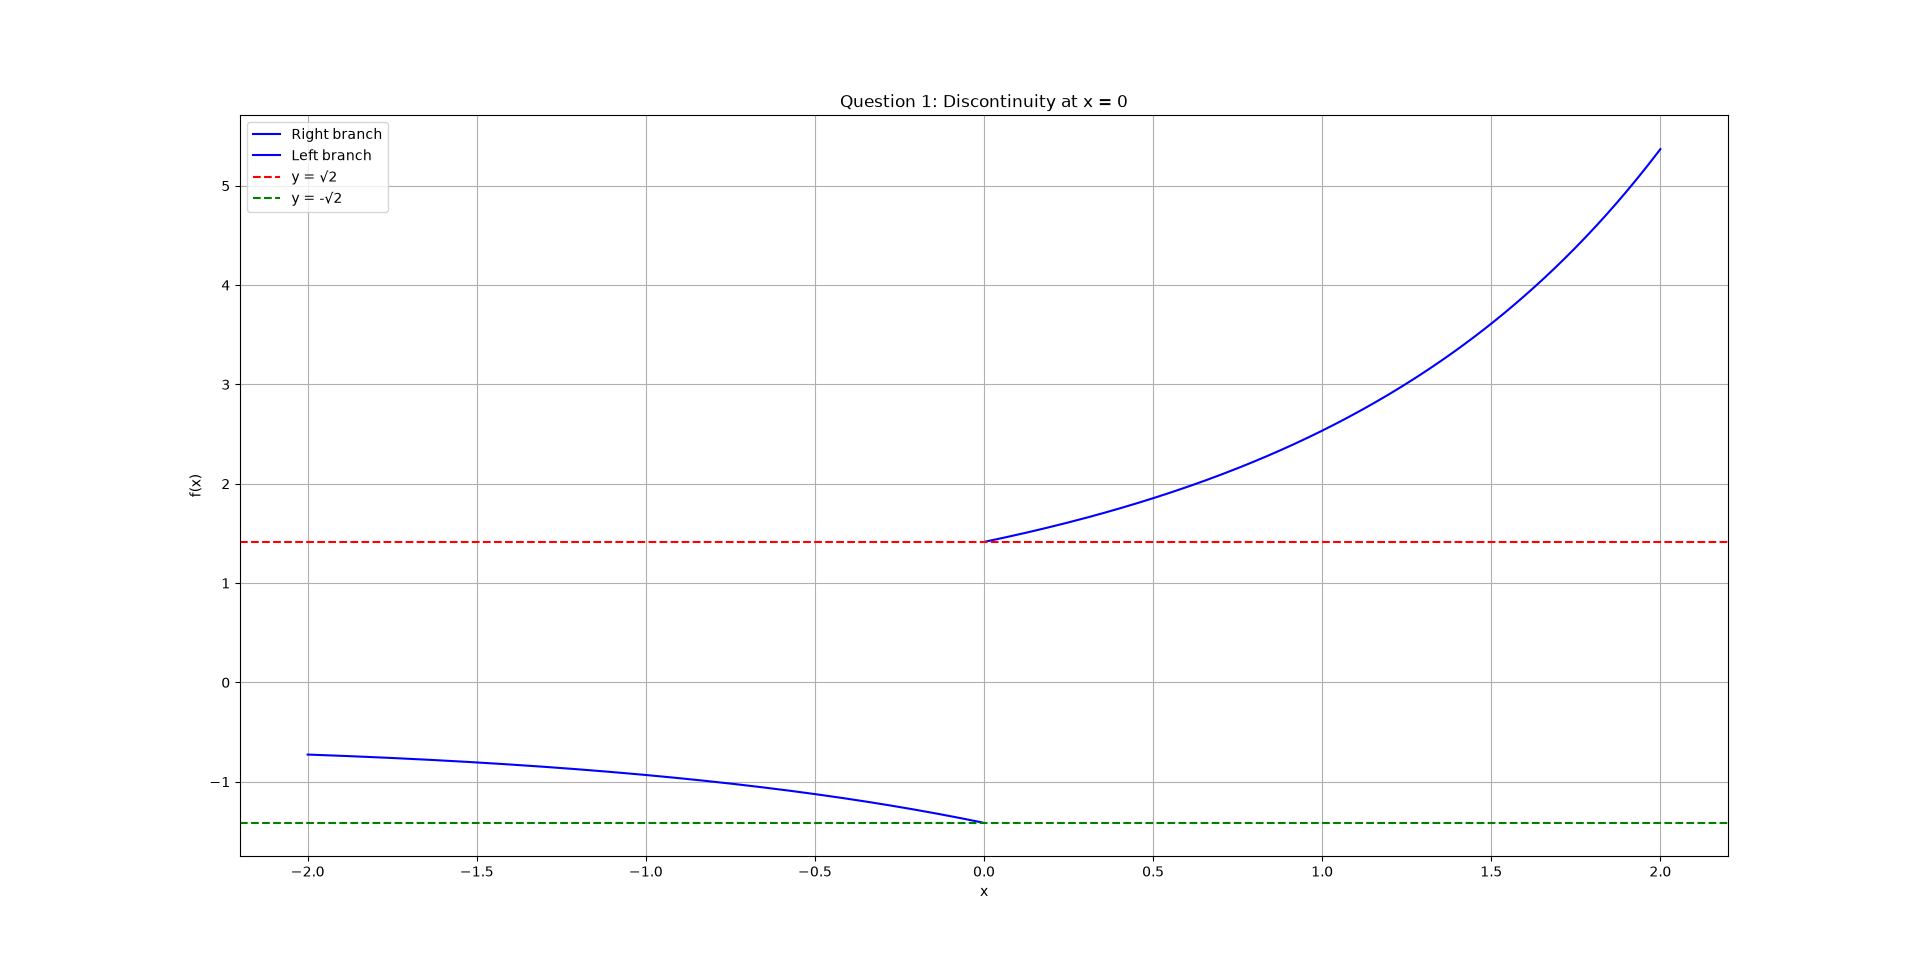
\includegraphics[width=0.9\textwidth]{figs/q1_fig}
		\caption{Discontinuity and one-sided limits at $x = 0$.}
		\label{fig:q1_fig}
		\vspace{0.5em}
		\noindent\fbox{\parbox{\dimexpr\textwidth-2\fboxsep-2\fboxrule}{\hspace{2em}\textbackslash codes\textbackslash q1.py}}
	\end{figure}
	
	\item Solve the differential equation $x\frac{dy}{dx} + y = x^3$, given $y=1$ when $x=2$. \hfill \brak{12, 2003}
	
	\solution
	From \eqref{eq:laplace_cauchy_euler}, substituting $x = 2e^t$ with $y\brak{0} = 1$ gives $\frac{dy}{dt} + y = 8e^{3t}u\brak{t}$. Taking the Laplace transform:
	\begin{align}
		\brak{sY\brak{s} - 1} + Y\brak{s} = \frac{8}{s-3} \implies Y\brak{s} = \frac{s+5}{\brak{s-3}\brak{s+1}} = \frac{2}{s-3} - \frac{1}{s+1}
	\end{align}
	From \eqref{eq:inv_laplace_pairs}, taking the inverse Laplace transform and substituting $t = \ln\brak{\frac{x}{2}}$:
	\begin{align}
		y\brak{t} &= \brak{2e^{3t} - e^{-t}}u\brak{t} \implies y\brak{x} = \frac{x^3}{4} - \frac{2}{x}, \quad x \ge 2
	\end{align}
	
	\item Given $\vec{A} = \myvec{3 & -2 \\ 4 & -2}$, find $k$ such that $\vec{A}^2 = k\vec{A} - 2\vec{I}_2$. \hfill \brak{12, 2003}
	
	\solution
	Computing $\vec{A}^2$:
	\begin{align}
		\vec{A}^2 = \myvec{3 & -2 \\ 4 & -2}\myvec{3 & -2 \\ 4 & -2} = \myvec{1 & -2 \\ 4 & -4}
	\end{align}
	By the Cayley-Hamilton theorem in \eqref{eq:cayley_hamilton_formula}:
	\begin{align}
		\vec{A}^2 - \text{Tr}\brak{\vec{A}}\vec{A} + \mydet{\vec{A}}\vec{I}_2 = \vec{0}
	\end{align}
	Evaluating the trace and determinant of $\vec{A}$:
	\begin{align}
		\text{Tr}\brak{\vec{A}} = 3 + \brak{-2} = 1, \quad \mydet{\vec{A}} = \brak{3}\brak{-2} - \brak{-2}\brak{4} = 2
	\end{align}
	Substituting these values:
	\begin{align}
		\vec{A}^2 - \vec{A} + 2\vec{I}_2 = \vec{0} \implies \vec{A}^2 = \vec{A} - 2\vec{I}_2
	\end{align}
	Comparing with $\vec{A}^2 = k\vec{A} - 2\vec{I}_2$ yields $k = 1$.
	
	\item Using the properties of determinants, show that:
	\begin{align*}
		\mydet{a+x & y & a+z \\ z & a+y & z \\ z & y & a+z} = a^2\brak{a+x+y+z}
	\end{align*}
	\hfill \brak{12, 2003}
	
	\solution
	By standard determinant operations referenced in \eqref{eq:det_prop_identity}:
	\begin{align}
		\mydet{a+x & y & a+z \\ z & a+y & z \\ z & y & a+z} 
		&\xrightarrow{R_1 \to R_1 + R_2 + R_3} \mydet{a+x+2z & a+2y & a+2z+y \\ z & a+y & z \\ z & y & a+z} \\
		&\xrightarrow[R_2 \to R_2 - R_3]{R_1 \to R_1 - R_3} \mydet{a+x & 0 & 0 \\ 0 & a & 0 \\ z & y & a+z} \\
		&= a^2\brak{a+x+y+z}
	\end{align}
	
	\item Find the intervals on which the function $f\brak{x} = \frac{x}{1+x^2}$ is
	
	(a) Increasing
	
	(b) Decreasing. \hfill \brak{12, 2003}
	
	\solution
	Differentiating $f\brak{x}$ with respect to $x$:
	\begin{align}
		f'\brak{x} = \frac{\brak{1+x^2}\brak{1} - x\brak{2x}}{\brak{1+x^2}^2} = \frac{1 - x^2}{\brak{1+x^2}^2}
	\end{align}
	Applying the monotonicity criteria from \eqref{eq:monotonicity_cond}:
	\begin{enumerate}[label=\brak{\alph*}]
		\item For $f\brak{x}$ to be increasing, $f'\brak{x} \ge 0 \implies 1 - x^2 \ge 0 \implies x \in \sbrak{-1, 1}$.
		\item For $f\brak{x}$ to be decreasing, $f'\brak{x} \le 0 \implies 1 - x^2 \le 0 \implies x \in \brak{-\infty, -1} \cup \brak{1, \infty}$.
	\end{enumerate}
	\begin{figure}[H]
		\centering
		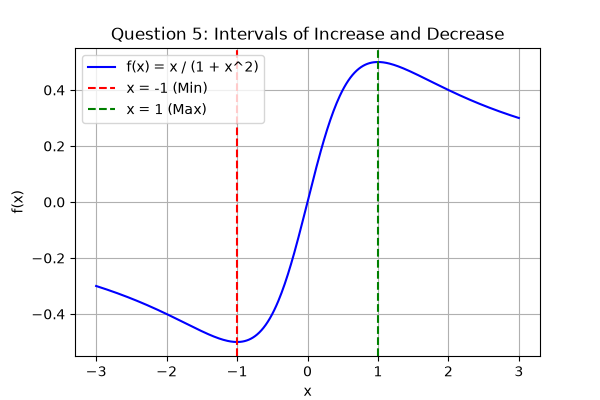
\includegraphics[width=0.6\textwidth]{figs/q5_fig}
		\caption{Intervals of increase and decrease for $f\brak{x} = \frac{x}{1+x^2}$.}
		\label{fig:q5_fig}
		\vspace{0.5em}
		\noindent\fbox{\parbox{\dimexpr\textwidth-2\fboxsep-2\fboxrule}{\hspace{2em}\textbackslash codes\textbackslash q5.py}}
	\end{figure}
	
	\item \hfill \brak{12, 2003}
	\begin{enumerate}[label=\brak{\alph*}]
		\item Approximate $I = \int_{0}^{\pi/2} \frac{\sin^2 x}{\sin x + \cos x} dx$ using the Trapezoidal Rule with $N=4$ subintervals.
		\item Approximate $I = \int_{0}^{\pi} \frac{x \sin x}{1 + \cos^2 x} dx$ using the Trapezoidal Rule with $N=4$ subintervals.
	\end{enumerate}
	\solution
	\begin{figure}[H]
		\centering
		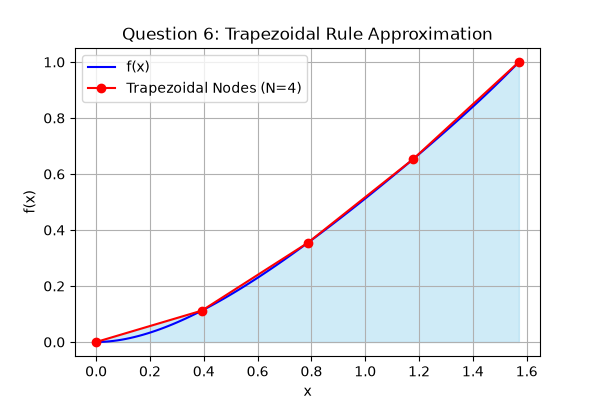
\includegraphics[width=0.7\textwidth]{figs/q6_fig}
		\caption{Trapezoidal Rule integration nodes.}
		\label{fig:q6_fig}
		\vspace{0.5em}
		\noindent\fbox{\parbox{\dimexpr\textwidth-2\fboxsep-2\fboxrule}{\hspace{2em}\textbackslash codes\textbackslash q6.py}}
	\end{figure}
	\begin{enumerate}[label=\brak{\alph*}]
		\item Applying the Trapezoidal Rule formula from \eqref{eq:trapezoidal_rule} with $h = \frac{\pi/2 - 0}{4} = \frac{\pi}{8}$:
		Evaluating $f\brak{x} = \frac{\sin^2 x}{\sin x + \cos x}$ at nodes $x_k = \frac{k\pi}{8}$ for $k=0,1,2,3,4$:
		\begin{align}
			y_0 &= f\brak{0} = 0, \quad y_1 = f\brak{\frac{\pi}{8}} \approx 0.1118 \\
			y_2 &= f\brak{\frac{\pi}{4}} \approx 0.3536, \quad y_3 = f\brak{\frac{3\pi}{8}} \approx 0.6010, \quad y_4 = f\brak{\frac{\pi}{2}} = 1.0000
		\end{align}
		Applying \eqref{eq:trapezoidal_rule}:
		\begin{align}
			I &\approx \frac{\pi}{16} \sbrak{y_0 + 2\brak{y_1 + y_2 + y_3} + y_4} \approx 0.6151
		\end{align}
		\item Applying \eqref{eq:trapezoidal_rule} with $h = \frac{\pi}{4}$:
		Evaluating $g\brak{x} = \frac{x\sin x}{1+\cos^2 x}$ at nodes $x_k = \frac{k\pi}{4}$ for $k=0,1,2,3,4$:
		\begin{align}
			y_0 = 0, \quad y_1 \approx 0.3702, \quad y_2 \approx 1.5708, \quad y_3 \approx 1.1107, \quad y_4 = 0
		\end{align}
		Applying \eqref{eq:trapezoidal_rule}:
		\begin{align}
			I &\approx \frac{\pi}{8} \sbrak{y_0 + 2\brak{y_1 + y_2 + y_3} + y_4} \approx 2.3968
		\end{align}
	\end{enumerate}
	
	\item Find Karl Pearson's coefficient of correlation between $x$ and $y$ for the given data vectors:
	\begin{align*}
		\vec{x} = \myvec{10 \\ 7 \\ 12 \\ 15 \\ 9 \\ 15 \\ 8}, \quad \vec{y} = \myvec{6 \\ 4 \\ 7 \\ 10 \\ 11 \\ 8 \\ 10}
	\end{align*}
	\hfill \brak{12, 2003}
	
	\solution
	Applying Karl Pearson's correlation coefficient in vector notation from \eqref{eq:karl_pearson_vec}:
	Computing the mean vectors using $\vec{1} = \myvec{1 & 1 & 1 & 1 & 1 & 1 & 1}^{\top}$:
	\begin{align}
		\bar{x} = \frac{\vec{1}^{\top}\vec{x}}{7} = \frac{76}{7} \approx 10.86, \quad \bar{y} = \frac{\vec{1}^{\top}\vec{y}}{7} = \frac{56}{7} = 8
	\end{align}
	Forming centered vectors $\vec{u} = \vec{x} - \bar{x}\vec{1}$ and $\vec{v} = \vec{y} - \bar{y}\vec{1}$:
	\begin{align}
		\vec{u}^{\top}\vec{v} = 22, \quad \norm{\vec{u}}^2 = 64.86, \quad \norm{\vec{v}}^2 = 42
	\end{align}
	Evaluating Karl Pearson's coefficient:
	\begin{align}
		r = \frac{\vec{u}^{\top}\vec{v}}{\norm{\vec{u}}\norm{\vec{v}}} = \frac{22}{\sqrt{64.86 \times 42}} \approx 0.421
	\end{align}
	
	\item A bag contains 8 red, 3 white, and 9 blue balls. If three balls are drawn at random, determine the probability that:
	
	(a) All three balls are blue
	
	(b) All balls are of different colors. \hfill \brak{12, 2003}
	
	\solution
	Expressing probability using Probability Mass Functions (PMF) $p_X\brak{k} = \pr{X = k}$ as per \eqref{eq:pmf_prob_def}:
	Total sample space size $N = \comb{20}{3} = 1140$.
	\begin{enumerate}[label=\brak{\alph*}]
		\item For $X = 3$ blue balls:
		\begin{align}
			p_X\brak{3} = \frac{\comb{9}{3}\comb{11}{0}}{\comb{20}{3}} = \frac{84}{1140} = \frac{7}{95} \approx 0.0737
		\end{align}
		\item For $Y = \brak{1\text{R}, 1\text{W}, 1\text{B}}$:
		\begin{align}
			p_Y\brak{1\text{R}, 1\text{W}, 1\text{B}} = \frac{\comb{8}{1} \times \comb{3}{1} \times \comb{9}{1}}{\comb{20}{3}} = \frac{216}{1140} = \frac{18}{95} \approx 0.1895
		\end{align}
	\end{enumerate}
	Monte Carlo simulation over $N_{\text{sim}} = 10^5$ trials yields empirical PMF estimates $\hat{p}_X\brak{3} \approx 0.0735$ and $\hat{p}_Y\brak{1\text{R}, 1\text{W}, 1\text{B}} \approx 0.1892$, closely matching the theoretical values.
	\begin{figure}[H]
		\centering
		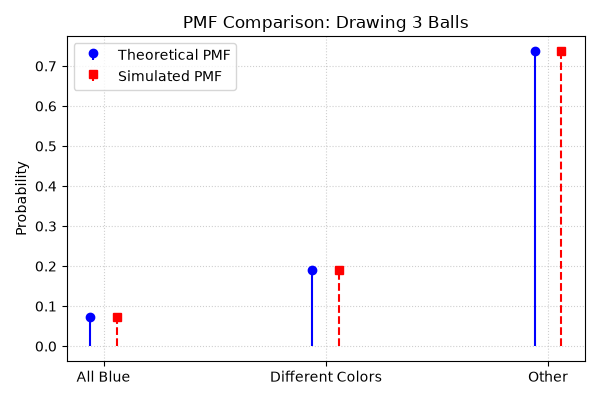
\includegraphics[width=0.65\textwidth]{figs/q8_fig}
		\caption{Theoretical vs. simulated PMF stem plot for ball draws.}
		\label{fig:q8_fig}
		\vspace{0.5em}
		\noindent\fbox{\parbox{\dimexpr\textwidth-2\fboxsep-2\fboxrule}{\hspace{2em}\textbackslash codes\textbackslash q8.py}}
	\end{figure}
	
	\item In a single throw of two dice, find the probability that neither a doublet nor a total of 10 will appear. \hfill \brak{12, 2003}
	
	\solution
	Define sample space size $N = 36$. Let $X = \mathbb{I}\brak{\text{doublet or sum}=10}$.
	Using PMF formulation from \eqref{eq:pmf_prob_def}:
	\begin{align}
		p_X\brak{1} = \pr{A \cup B} = \frac{6}{36} + \frac{3}{36} - \frac{1}{36} = \frac{8}{36} = \frac{2}{9} \approx 0.2222
	\end{align}
	The PMF for neither event occurring ($X = 0$) is:
	\begin{align}
		p_X\brak{0} = 1 - p_X\brak{1} = 1 - \frac{2}{9} = \frac{7}{9} \approx 0.7778
	\end{align}
	Simulating $N_{\text{sim}} = 10^5$ throws of two dice yields $\hat{p}_X\brak{0} \approx 0.7781$ and $\hat{p}_X\brak{1} \approx 0.2219$, confirming the analytical PMF.
	\begin{figure}[H]
		\centering
		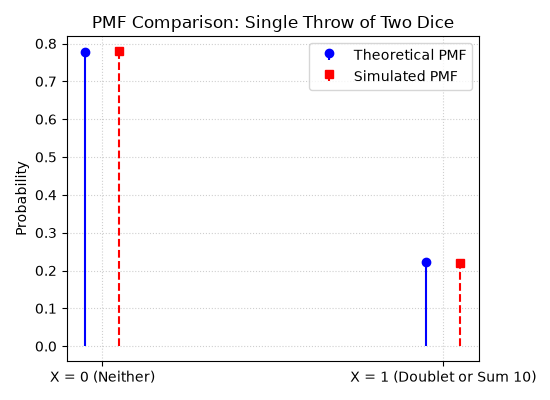
\includegraphics[width=0.65\textwidth]{figs/q9_fig}
		\caption{Theoretical vs. simulated PMF stem plot for two-dice throws.}
		\label{fig:q9_fig}
		\vspace{0.5em}
		\noindent\fbox{\parbox{\dimexpr\textwidth-2\fboxsep-2\fboxrule}{\hspace{2em}\textbackslash codes\textbackslash q9.py}}
	\end{figure}
	
	\item Using Gauss Elimination method, solve the system of linear equations:
	\begin{align*}
		2x - y + z &= -3 \\
		3x - z &= -8 \\
		2x + 6y &= 2
	\end{align*}
	\hfill \brak{12, 2003}
	
	\solution
	Constructing the augmented matrix $\augvec{3}{1}{2 & -1 & 1 & -3 \\ 3 & 0 & -1 & -8 \\ 2 & 6 & 0 & 2}$ as defined in \eqref{eq:gauss_elimination_def}:
	\begin{align}
		\left[\begin{array}{ccc|c}
			2 & -1 & 1 & -3 \\
			3 & 0 & -1 & -8 \\
			2 & 6 & 0 & 2
		\end{array}\right]
		&\xrightarrow[R_3 \to R_3 - R_1]{R_2 \to R_2 - \frac{3}{2}R_1}
		\left[\begin{array}{ccc|c}
			2 & -1 & 1 & -3 \\
			0 & 1.5 & -2.5 & -3.5 \\
			0 & 7 & -1 & 5
		\end{array}\right] \nonumber \\
		&\xrightarrow{R_3 \to R_3 - \frac{14}{3}R_2}
		\left[\begin{array}{ccc|c}
			2 & -1 & 1 & -3 \\
			0 & 1.5 & -2.5 & -3.5 \\
			0 & 0 & \frac{32}{3} & \frac{64}{3}
		\end{array}\right]
	\end{align}
	Back-substitution yields $z = 2, y = 1, x = -2 \implies \vec{x} = \myvec{-2 \\ 1 \\ 2}$.
	
	\item Prove that the area enclosed by $y^2 = 4ax$ and $x^2 = 4ay$ is $\frac{16}{3}a^2$ square units. \hfill \brak{12, 2003}
	
	\solution
	\begin{figure}[H]
		\centering
		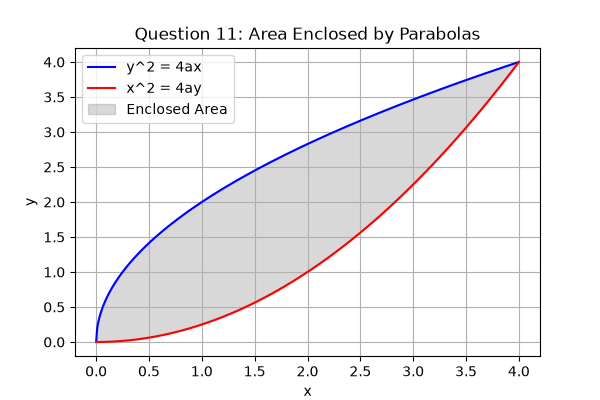
\includegraphics[width=0.7\textwidth]{figs/q11_fig}
		\caption{Area enclosed between the parabolas $y^2 = 4ax$ and $x^2 = 4ay$.}
		\label{fig:q11_fig}
		\vspace{0.5em}
		\noindent\fbox{\parbox{\dimexpr\textwidth-2\fboxsep-2\fboxrule}{\hspace{2em}\textbackslash codes\textbackslash q11.py}}
	\end{figure}  
	Expressing the two parabolas $y^2 - 4ax = 0$ and $x^2 - 4ay = 0$ in matrix form $\vec{x}^{\top}\vec{V}_i\vec{x} + 2\vec{u}_i^{\top}\vec{x} + f_i = 0$:
	\begin{align}
		\vec{V}_1 = \myvec{0 & 0 \\ 0 & 1}, \quad \vec{u}_1 = \myvec{-2a \\ 0}, \quad f_1 = 0; \qquad \vec{V}_2 = \myvec{1 & 0 \\ 0 & 0}, \quad \vec{u}_2 = \myvec{0 \\ -2a}, \quad f_2 = 0
	\end{align}
	From \eqref{eq:pencil_conics} and \eqref{eq:degenerate_conic_det}, the pencil of conics degenerates into a pair of straight lines when:
	\begin{align}
		\mydet{\mu & 0 & -2a \\ 0 & 1 & -2a\mu \\ -2a & -2a\mu & 0} = 0 \implies -4a^2\brak{1 + \mu^3} = 0 \implies \mu = -1
	\end{align}
	Substituting $\mu = -1$ into \eqref{eq:pencil_conics} yields the chord pair $\brak{y - x}\brak{y + x + 4a} = 0$. Intersecting $y = x$ with $y^2 = 4ax$ gives $x^2 = 4ax \implies x = 0, \, x = 4a$ (while $y + x + 4a = 0$ gives no real intersection).
	
	From \eqref{eq:area_between_curves}, the area enclosed between $x = 0$ and $x = 4a$ is:
	\begin{align}
		\text{Area} &= \int_{0}^{4a} \brak{\sqrt{4ax} - \frac{x^2}{4a}} dx = \sbrak{2\sqrt{a}\cdot\frac{2}{3}x^{3/2} - \frac{x^3}{12a}}_{0}^{4a} \nonumber \\
		&= \frac{4}{3}\sqrt{a}\brak{8a^{3/2}} - \frac{64a^3}{12a} = \frac{32}{3}a^2 - \frac{16}{3}a^2 = \frac{16}{3}a^2 \quad \text{sq. units} \label{eq:area_parabolas}
	\end{align}
	
	\item \hfill \brak{12, 2003}
	\begin{enumerate}[label=\brak{\alph*}]
		\item Using vectors prove that $\cos A = \frac{b^2 + c^2 - a^2}{2bc}$.
		\item Three bags contain balls as shown in the following table:
		\begin{center}
			\begin{tabular}{|c|c|c|c|}
				\hline
				Bag & \multicolumn{3}{c|}{Number of} \\ \hline
				& White balls & Black balls & Red balls \\ \hline
				I & 1 & 2 & 3 \\
				II & 2 & 1 & 1 \\
				III & 4 & 3 & 2 \\ \hline
			\end{tabular}
		\end{center}
		A bag is chosen at random and two balls are drawn. They happen to be white and red. What is the probability that they came from the third bag?
	\end{enumerate}
	\solution
	\begin{enumerate}[label=\brak{\alph*}]
		\item Assuming vertex coordinates $\vec{A} = \myvec{0 \\ 0}$ and $\vec{B} = \myvec{c \\ 0}$ with side lengths $\norm{\vec{B} - \vec{C}} = a$, $\norm{\vec{C} - \vec{A}} = b$, and interior angle $A$ at $\vec{A}$, vertex $\vec{C}$ is derived as $\vec{C} = \myvec{b\cos A \\ b\sin A}$. Defining the cyclic side vectors $\vec{c} = \vec{B} - \vec{A} = \myvec{c \\ 0}$, $\vec{b} = \vec{A} - \vec{C} = \myvec{-b\cos A \\ -b\sin A}$, and $\vec{a} = \vec{C} - \vec{B} = \myvec{b\cos A - c \\ b\sin A}$, we verify $\vec{a} + \vec{b} + \vec{c} = \vec{0} \implies \vec{a} = -\brak{\vec{b} + \vec{c}}$. From \eqref{eq:vector_dot_cosine}:
		\begin{align}
			\norm{\vec{a}}^2 &= \brak{\vec{b} + \vec{c}}^{\top}\brak{\vec{b} + \vec{c}} \\
			a^2 &= \norm{\vec{b}}^2 + \norm{\vec{c}}^2 + 2\vec{b}^{\top}\vec{c} \\
			a^2 &= b^2 + c^2 - 2bc\cos A \implies \cos A = \frac{b^2 + c^2 - a^2}{2bc}
		\end{align}
		\begin{figure}[H]
			\centering
			\includegraphics[width=0.6\textwidth]{figs/q12a_fig}
			\caption{Vector representation of triangle $ABC$ in coordinate space.}
			\label{fig:q12a_fig}
			\vspace{0.5em}
			\noindent\fbox{\parbox{\dimexpr\textwidth-2\fboxsep-2\fboxrule}{\hspace{2em}\textbackslash codes\textbackslash 12a.py}}
		\end{figure}
		\item Prior PMF $p_B\brak{1} = p_B\brak{2} = p_B\brak{3} = \frac{1}{3}$.
		Conditional PMFs for drawing 1 white and 1 red ball $E$:
		\begin{align}
			p_{E|B}\brak{e|1} = \frac{1}{5}, \quad p_{E|B}\brak{e|2} = \frac{1}{3}, \quad p_{E|B}\brak{e|3} = \frac{2}{9}
		\end{align}
		From \eqref{eq:posterior_pmf_formula}, the posterior PMF is:
		\begin{align}
			p_{B|E}\brak{3|e} = \frac{\frac{1}{3} \times \frac{2}{9}}{\frac{1}{3}\brak{\frac{1}{5} + \frac{1}{3} + \frac{2}{9}}} = \frac{\frac{2}{9}}{\frac{34}{45}} = \frac{5}{17} \approx 0.2941
		\end{align}
		Monte Carlo simulation over $N_{\text{sim}} = 10^5$ trials gives posterior estimates $\hat{p}_{B|E}\brak{1|e} \approx 0.2645$, $\hat{p}_{B|E}\brak{2|e} \approx 0.4410$, and $\hat{p}_{B|E}\brak{3|e} \approx 0.2945$, matching the exact values $\frac{9}{34}, \frac{15}{34}, \frac{5}{17}$.
		\begin{figure}[H]
			\centering
			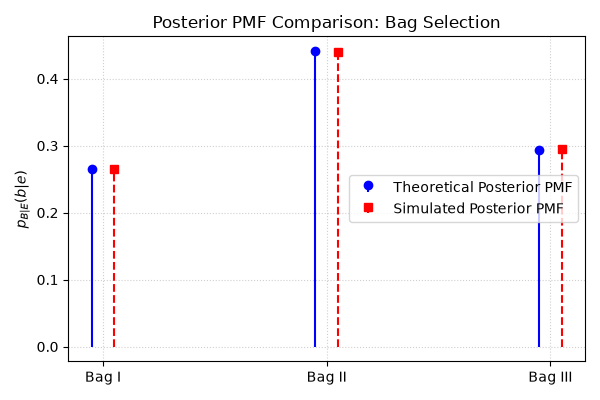
\includegraphics[width=0.65\textwidth]{figs/q12b_fig}
			\caption{Theoretical vs. simulated posterior PMF stem plot for bag selection.}
			\label{fig:q12b_fig}
			\vspace{0.5em}
			\noindent\fbox{\parbox{\dimexpr\textwidth-2\fboxsep-2\fboxrule}{\hspace{2em}\textbackslash codes\textbackslash 12b.py}}
		\end{figure}
	\end{enumerate}
	
	\item The first four moments of a distribution about $x=2$ are $1, 2.5, 5.5$, and $16$ respectively. Calculate the four moments about the mean. \hfill \brak{12, 2003}
	
	\solution
	Given raw moments $\mu_1' = 1, \mu_2' = 2.5, \mu_3' = 5.5, \mu_4' = 16$ about $A = 2$.
	The central moments $\mu_r$ about the mean are:
	\begin{align}
		\mu_1 &= 0 \\
		\mu_2 &= \mu_2' - \brak{\mu_1'}^2 = 2.5 - \brak{1}^2 = 1.5 \\
		\mu_3 &= \mu_3' - 3\mu_2'\mu_1' + 2\brak{\mu_1'}^3 = 5.5 - 7.5 + 2 = 0 \\
		\mu_4 &= \mu_4' - 4\mu_3'\mu_1' + 6\mu_2'\brak{\mu_1'}^2 - 3\brak{\mu_1'}^4 = 16 - 22 + 15 - 3 = 6
	\end{align}
	Central moments: $\mu_1 = 0, \mu_2 = 1.5, \mu_3 = 0, \mu_4 = 6$.
	
	\item \hfill \brak{12, 2003}
	\begin{enumerate}[label=\brak{\alph*}]
		\item A particle is projected so as to graze the tops of two walls, each of height $10\text{ m}$ at distances $15\text{ m}$ and $45\text{ m}$ respectively from the point of projection. Prove that the angle of projection is $\tan^{-1}\brak{\frac{8}{9}}$.
		\item A starts a business with a capital of Rs. $4,00,000$. After 3 months B joins him with a capital of Rs. $6,00,000$ and at the end of another 3 months C joins with Rs. $10,00,000$. If at the end of the year, the total profit be Rs. $5,40,000$, and they share it in the ratio of their effective capitals, calculate the shares of A, B and C in the total profit.
	\end{enumerate}
	\solution
	\begin{enumerate}[label=\brak{\alph*}]
		\item Using the trajectory formula from \eqref{eq:projectile_trajectory}:
		Since the particle grazes two walls of height $h = 10\text{ m}$ at $x_1 = 15\text{ m}$ and $x_2 = 45\text{ m}$:
		\begin{align}
			10 &= 15 \tan\theta \brak{1 - \frac{15}{R}} \label{eq:wall1} \\
			10 &= 45 \tan\theta \brak{1 - \frac{45}{R}} \label{eq:wall2}
		\end{align}
		Equating \eqref{eq:wall1} and \eqref{eq:wall2}:
		\begin{align}
			15 \brak{1 - \frac{15}{R}} = 45 \brak{1 - \frac{45}{R}} \implies 1 - \frac{15}{R} = 3 - \frac{135}{R} \implies \frac{120}{R} = 2 \implies R = 60\text{ m}
		\end{align}
		Substituting $R = 60\text{ m}$ into \eqref{eq:wall1}:
		\begin{align}
			10 = 15 \tan\theta \brak{1 - \frac{15}{60}} = 15 \tan\theta \brak{\frac{3}{4}} = \frac{45}{4}\tan\theta \implies \tan\theta = \frac{40}{45} = \frac{8}{9}
		\end{align}
		Thus, the angle of projection is $\theta = \tan^{-1}\brak{\frac{8}{9}}$.
		\begin{figure}[H]
			\centering
			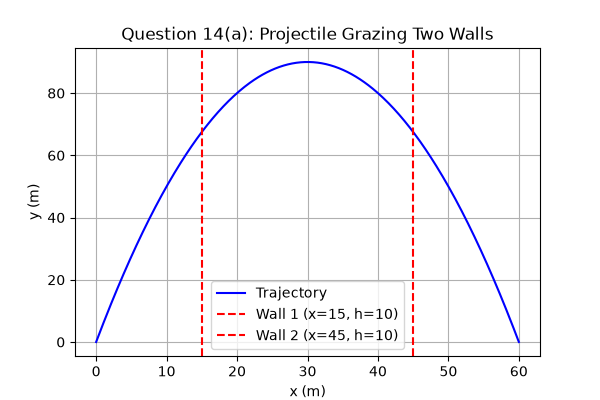
\includegraphics[width=0.7\textwidth]{figs/q14_fig}
			\caption{Projectile trajectory grazing two walls.}
			\label{fig:q14_fig}
			\vspace{0.5em}
			\noindent\fbox{\parbox{\dimexpr\textwidth-2\fboxsep-2\fboxrule}{\hspace{2em}\textbackslash codes\textbackslash q14.py}}
		\end{figure}
		\item Given capital vector $\vec{k} = \myvec{4,00,000 \\ 6,00,000 \\ 10,00,000}$ and duration vector $\vec{t} = \myvec{12 \\ 9 \\ 6}$, from \eqref{eq:partnership_profit_vec}, the effective capital-months vector is $\vec{c} = \vec{k} \odot \vec{t} = \myvec{48,00,000 \\ 54,00,000 \\ 60,00,000} \implies \vec{r} = \myvec{8 \\ 9 \\ 10}$.
		With sum of ratio terms $\vec{1}^{\top}\vec{r} = 27$ and total profit $P = 5,40,000$, the profit vector is:
		\begin{align}
			\vec{p} = \frac{5,40,000}{27}\myvec{8 \\ 9 \\ 10} = \myvec{1,60,000 \\ 1,80,000 \\ 2,00,000}
		\end{align}
		Shares: A $=$ Rs. $1,60,000$, B $=$ Rs. $1,80,000$, C $=$ Rs. $2,00,000$.
		\begin{figure}[H]
			\centering
			\noindent\fbox{\parbox{\dimexpr\textwidth-2\fboxsep-2\fboxrule}{\hspace{2em}\textbackslash codes\textbackslash 14b.c}}
		\end{figure}
	\end{enumerate}
	
	\item \hfill \brak{12, 2003}
	\begin{enumerate}[label=\brak{\alph*}]
		\item A stone is projected vertically upward with a velocity sufficient to carry it to a height of $50\text{ m}$. Find its velocity of projection and the time taken to come back to the ground. [Use $g = 9.8\text{ m/s}^2$]
		\item The cost function of a firm is given by $C\brak{x} = 300x - 10x^2 + \frac{x^3}{3}$. Calculate the output at which the marginal cost is minimum. Also calculate the minimum marginal cost.
	\end{enumerate}
	\solution
	\begin{enumerate}[label=\brak{\alph*}]
		\item Given maximum height $H = 50\text{ m}$ and acceleration due to gravity $g = 9.8\text{ m/s}^2$, from \eqref{eq:vertical_motion_gravity}, the velocity of projection $u$ is:
		\begin{align}
			u = \sqrt{2\brak{9.8}\brak{50}} = \sqrt{980} = 14\sqrt{5} \approx 31.30\text{ m/s}
		\end{align}
		From \eqref{eq:vertical_motion_gravity}, the total time taken to return to the ground (time of flight $T$) is:
		\begin{align}
			T = \frac{2 \times 31.3049}{9.8} \approx 6.39\text{ seconds}
		\end{align}
		\begin{figure}[H]
			\centering
			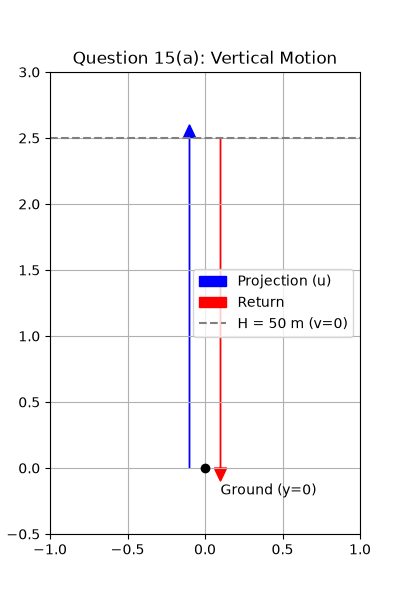
\includegraphics[width=0.5\textwidth]{figs/q15_fig}
			\caption{Vertical motion under gravity.}
			\label{fig:q15_fig}
			\vspace{0.5em}
			\noindent\fbox{\parbox{\dimexpr\textwidth-2\fboxsep-2\fboxrule}{\hspace{2em}\textbackslash codes\textbackslash q15.py}}
		\end{figure}
		\item Marginal cost is $MC\brak{x} = \frac{dC}{dx} = 300 - 20x + x^2$, so $f\brak{x} = MC'\brak{x} = -20 + 2x$ and $f'\brak{x} = MC''\brak{x} = 2$. Applying the Newton-Raphson update from \eqref{eq:newton_raphson_opt} starting at $x_0 = 0$:
		\begin{align}
			x_1 = x_0 - \frac{-20 + 2x_0}{2} = 0 - \frac{-20}{2} = 10
		\end{align}
		Since $MC''\brak{10} = 2 > 0$, $MC\brak{x}$ attains its minimum at $x = 10$:
		\begin{align}
			MC_{\text{min}} = 300 - 20\brak{10} + \brak{10}^2 = 200
		\end{align}
		\begin{figure}[H]
			\centering
			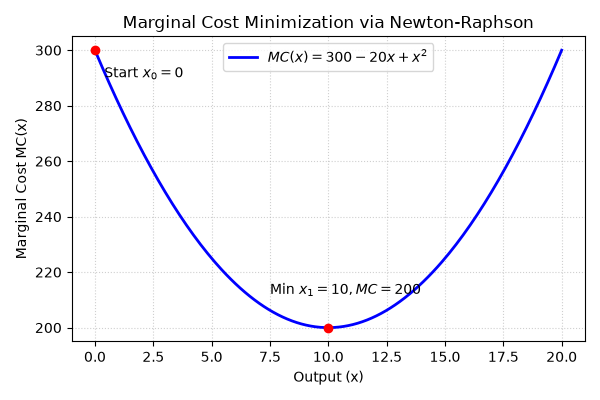
\includegraphics[width=0.6\textwidth]{figs/q15b_fig}
			\caption{Marginal cost minimization via Newton-Raphson method.}
			\label{fig:q15b_fig}
			\vspace{0.5em}
			\noindent\fbox{\parbox{\dimexpr\textwidth-2\fboxsep-2\fboxrule}{\hspace{2em}\textbackslash codes\textbackslash 15b.py}}
		\end{figure}
	\end{enumerate}
	
	\item \hfill \brak{12, 2003}
	\begin{enumerate}[label=\brak{\alph*}]
		\item Solve the differential equation $\frac{d^2y}{dx^2} = \log x$, given that $x=1, y=1 \text{ and } \frac{dy}{dx} = 1$.
		\item Calculate Bowley's coefficient of skewness for the given frequency distribution:
		\begin{center}
			\begin{tabular}{|c|c|c|c|c|c|c|c|c|c|}
				\hline
				x & 5 & 10 & 15 & 20 & 25 & 30 & 35 & 40 & 45 \\ \hline
				y & 9 & 8 & 12 & 15 & 11 & 7 & 6 & 5 & 2 \\ \hline
			\end{tabular}
		\end{center}
	\end{enumerate}
	\solution
	\begin{enumerate}[label=\brak{\alph*}]
		\item From \eqref{eq:laplace_second_order}, substituting $x = e^t$ ($t = \ln x$) converts the initial conditions at $x = 1$ ($t = 0$) to $y\brak{0} = 1$ and $y'\brak{0} = \left.e^t\frac{dy}{dx}\right|_{t=0} = 1$, giving:
		\begin{align}
			e^{-2t}\brak{\frac{d^2y}{dt^2} - \frac{dy}{dt}} = t\,u\brak{t} \implies \frac{d^2y}{dt^2} - \frac{dy}{dt} = t e^{2t} u\brak{t}
		\end{align}
		Taking the Laplace transform using \eqref{eq:laplace_cauchy_euler} and \eqref{eq:laplace_second_order}:
		\begin{align}
			\brak{s^2 Y\brak{s} - s\brak{1} - 1} - \brak{s Y\brak{s} - 1} &= \frac{1}{\brak{s-2}^2} \\
			s\brak{s-1}Y\brak{s} &= s + \frac{1}{\brak{s-2}^2} \implies Y\brak{s} = \frac{1}{s-1} + \frac{1}{s\brak{s-1}\brak{s-2}^2}
		\end{align}
		Resolving into partial fractions:
		\begin{align}
			Y\brak{s} = -\frac{1}{4s} + \frac{2}{s-1} - \frac{3}{4\brak{s-2}} + \frac{1}{2\brak{s-2}^2}
		\end{align}
		Applying the inverse Laplace transform from \eqref{eq:inv_laplace_pairs} and \eqref{eq:laplace_second_order}:
		\begin{align}
			y\brak{t} = \brak{-\frac{1}{4} + 2e^t - \frac{3}{4}e^{2t} + \frac{1}{2}t e^{2t}}u\brak{t}
		\end{align}
		Substituting $t = \ln x$ ($e^t = x$, $x \ge 1$) yields:
		\begin{align}
			y\brak{x} = \frac{x^2}{2}\log x - \frac{3x^2}{4} + 2x - \frac{1}{4}, \quad x \ge 1
		\end{align}
		\item Constructing cumulative frequency ($N = 75$):
		Quartile positions give $Q_1 = 15, Q_2 = 20, Q_3 = 30$.
		From \eqref{eq:bowley_skewness}, Bowley's coefficient is:
		\begin{align}
			S_b = \frac{30 + 15 - 40}{30 - 15} = \frac{5}{15} = \frac{1}{3} \approx 0.333
		\end{align}
	\end{enumerate}
	
	\item \hfill \brak{12, 2003}
	\begin{enumerate}[label=\brak{\alph*}]
		\item The Cartesian equations of a line are $6x - 2 = 3y + 1 = 2z - 2$. Find:
		\begin{enumerate}[label=\brak{\roman*}]
			\item The direction ratios of the line.
			\item Cartesian and vector equations of the line parallel to this line and passing through the point $\brak{2, -1, -1}$.
		\end{enumerate}
		\item Find the present value of an ordinary annuity of Rs. $500$ per annum for $12$ years at $15\%$ per annum. [Given $\brak{1.15}^{-12} = \frac{1}{5.35}$]
	\end{enumerate}
	\solution
	\begin{enumerate}[label=\brak{\alph*}]
		\item Rewriting the given line equation $6x - 2 = 3y + 1 = 2z - 2$ in standard symmetric form \eqref{eq:line_3d_symmetric_vec}:
		Dividing each term by $\text{LCM}\brak{6, 3, 2} = 6$:
		\begin{align}
			\frac{6\brak{x - \frac{1}{3}}}{6} = \frac{3\brak{y + \frac{1}{3}}}{6} = \frac{2\brak{z - 1}}{6} \implies \frac{x - \frac{1}{3}}{1} = \frac{y + \frac{1}{3}}{2} = \frac{z - 1}{3}
		\end{align}
		\begin{enumerate}[label=\brak{\roman*}]
			\item The direction ratios of the line are the denominators $\brak{1, 2, 3}$, or as a vector $\vec{m} = \myvec{1 \\ 2 \\ 3}$.
			\item For a line parallel to this line and passing through $\vec{x}_0 = \myvec{2 \\ -1 \\ -1}$:
			\begin{itemize}
				\item \textbf{Cartesian Equation:}
				\begin{align}
					\frac{x - 2}{1} = \frac{y + 1}{2} = \frac{z + 1}{3}
				\end{align}
				\item \textbf{Vector Equation:}
				\begin{align}
					\vec{r} = \myvec{2 \\ -1 \\ -1} + \lambda \myvec{1 \\ 2 \\ 3}, \quad \lambda \in \mathbb{R}
				\end{align}
			\end{itemize}
		\end{enumerate}
		\begin{figure}[H]
			\centering
			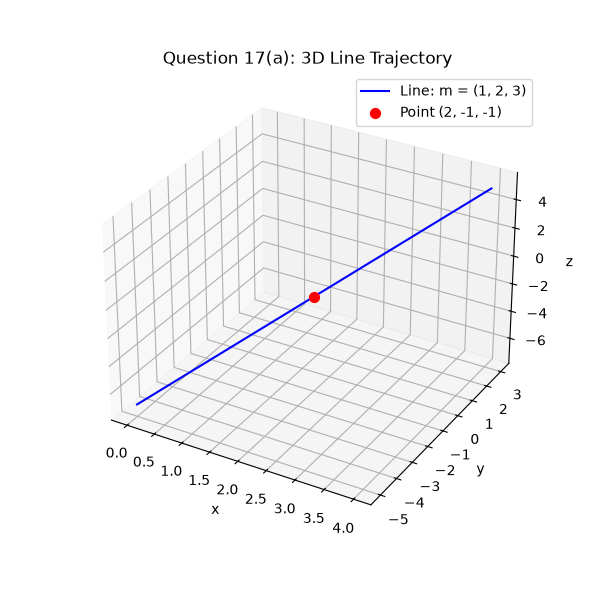
\includegraphics[width=0.6\textwidth]{figs/q17_fig}
			\caption{3D line direction and point representation.}
			\label{fig:q17_fig}
			\vspace{0.5em}
			\noindent\fbox{\parbox{\dimexpr\textwidth-2\fboxsep-2\fboxrule}{\hspace{2em}\textbackslash codes\textbackslash q17.py}}
		\end{figure}
		\item Present value formula from \eqref{eq:annuity_pv_formula} by substituting $R = 500, i = 0.15, \brak{1.15}^{-12} \approx 0.1869$:
		\begin{align}
			P = 500 \sbrak{\frac{1 - 0.1869}{0.15}} = 500 \times 5.4206 = \text{Rs. } 2710.30
		\end{align}
		\begin{figure}[H]
			\centering
			\noindent\fbox{\parbox{\dimexpr\textwidth-2\fboxsep-2\fboxrule}{\hspace{2em}\textbackslash codes\textbackslash 17b.c}}
		\end{figure}
	\end{enumerate}
	
	\item \hfill \brak{12, 2003}
	\begin{enumerate}[label=\brak{\alph*}]
		\item If the plane $x + y + z = \sqrt{3}\lambda$ touches the sphere $x^2 + y^2 + z^2 - 2x - 2z - 6 = 0$, find the value of $\lambda$.
		\item An insurance company discovers $0.1\%$ of the population is involved in accidents. For 1000 policy holders, find the probability that not more than 5 are involved next year. [Use $e^{-1} = 0.368$]
	\end{enumerate}
	\solution
	\begin{enumerate}[label=\brak{\alph*}]
		\item Expressing the sphere $x^2 + y^2 + z^2 - 2x - 2z - 6 = 0$ in matrix form $g\brak{\vec{x}} = \vec{x}^{\top}\vec{V}\vec{x} + 2\vec{u}^{\top}\vec{x} + f = 0$:
		\begin{align}
			\vec{V} = \vec{I}_3, \quad \vec{u} = \myvec{-1 \\ 0 \\ -1}, \quad f = -6
		\end{align}
		The line through center $\vec{h} = -\vec{u} = \myvec{1 \\ 0 \\ 1}$ along the plane's normal $\vec{m} = \myvec{1 \\ 1 \\ 1}$ is $\vec{x} = \vec{h} + \kappa\vec{m}$. From \eqref{eq:line_conic_inter}, the points of intersection of this normal line with the sphere are given by:
		\begin{align}
			\kappa_i = \frac{1}{\vec{m}^{\top}\vec{V}\vec{m}}\brak{-\vec{m}^{\top}\brak{\vec{V}\vec{h} + \vec{u}} \pm \sqrt{\sbrak{\vec{m}^{\top}\brak{\vec{V}\vec{h} + \vec{u}}}^2 - g\brak{\vec{h}}\brak{\vec{m}^{\top}\vec{V}\vec{m}}}}
		\end{align}
		Evaluating the terms: $\vec{V}\vec{h} + \vec{u} = \vec{0}$, $\vec{m}^{\top}\vec{V}\vec{m} = 3$, and $g\brak{\vec{h}} = \norm{\vec{h}}^2 + 2\vec{u}^{\top}\vec{h} + f = 2 - 4 - 6 = -8$:
		\begin{align}
			\kappa_i = \frac{1}{3}\brak{0 \pm \sqrt{0 - \brak{-8}\brak{3}}} = \pm\frac{2\sqrt{6}}{3} \implies \vec{x}_i = \myvec{1 \\ 0 \\ 1} \pm \frac{2\sqrt{6}}{3}\myvec{1 \\ 1 \\ 1}
		\end{align}
		Since the plane $\vec{m}^{\top}\vec{x} = \sqrt{3}\lambda$ touches the sphere at $\vec{x}_i$, substituting $\vec{x}_i$ into the plane equation yields:
		\begin{align}
			\vec{m}^{\top}\vec{h} + \kappa_i\brak{\vec{m}^{\top}\vec{m}} = \sqrt{3}\lambda \implies 2 \pm 2\sqrt{6} = \sqrt{3}\lambda \implies \lambda = \frac{2\sqrt{3} \pm 6\sqrt{2}}{3}
		\end{align}
		\begin{figure}[H]
			\centering
			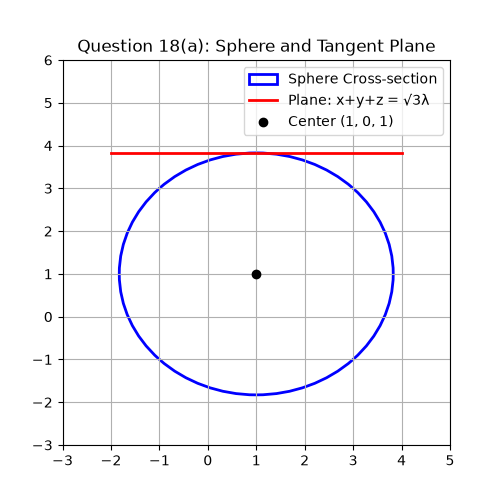
\includegraphics[width=0.6\textwidth]{figs/q18_fig}
			\caption{Sphere and tangent plane representation.}
			\label{fig:q18_fig}
			\vspace{0.5em}
			\noindent\fbox{\parbox{\dimexpr\textwidth-2\fboxsep-2\fboxrule}{\hspace{2em}\textbackslash codes\textbackslash q18.py}}
		\end{figure}
		\item Poisson PMF from \eqref{eq:poisson_pmf_formula} with $\lambda_{P} = np = 1000 \times 0.001 = 1$:
		\begin{align}
			p_X\brak{X \le 5} = \sum_{k=0}^{5} \frac{0.368}{k!} = 0.368 \times 2.7167 \approx 0.9997
		\end{align}
		Monte Carlo simulation of $N_{\text{sim}} = 10^5$ policy cohorts gives $\hat{p}_X\brak{X \le 5} \approx 0.9994$, closely matching the Poisson PMF stem distribution.
		\begin{figure}[H]
			\centering
			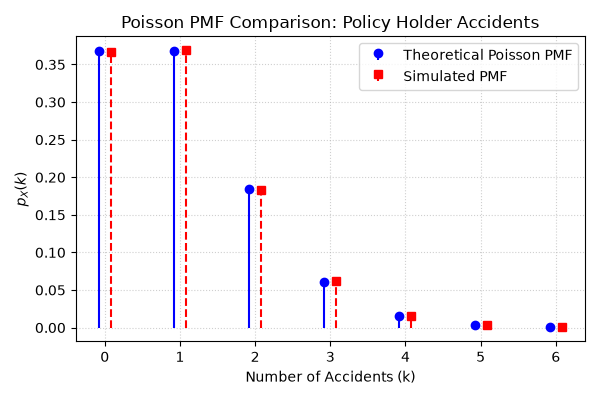
\includegraphics[width=0.65\textwidth]{figs/q18b_fig}
			\caption{Theoretical vs. simulated Poisson PMF stem plot for accident claims.}
			\label{fig:q18b_fig}
			\vspace{0.5em}
			\noindent\fbox{\parbox{\dimexpr\textwidth-2\fboxsep-2\fboxrule}{\hspace{2em}\textbackslash codes\textbackslash 18b.py}}
		\end{figure}
	\end{enumerate}
	
	\item \hfill \brak{12, 2003}
	\begin{enumerate}[label=\brak{\alph*}]
		\item Three forces $\vec{P}, \vec{Q}$ and $\vec{R}$ acting at a point are in equilibrium. The angle between $\vec{P}$ and $\vec{R}$ is double the angle between $\vec{P}$ and $\vec{Q}$. Prove that $R^2 = Q\brak{Q-P}$.
		\item The horizontal roadway of a bridge $AB$, $12\text{ m}$ long, weight $56000\text{ N}$ and rests on two supports at its ends. What is the pressure on each support when a lorry of weight $33600\text{ N}$, starting from $A$, is at a point two-third of the way on the bridge?
		\item A housewife wishes to mix up two kinds of foods $X$ and $Y$ in such a way that mixture contains at least 10 units of vitamin A, 12 units of vitamin B and 8 units of vitamin C.
		\begin{center}
			\begin{tabular}{|c|c|c|c|}
				\hline
				Food & Vitamin A & Vitamin B & Vitamin C \\ \hline
				X & 1 & 2 & 3 \\
				Y & 2 & 2 & 1 \\ \hline
			\end{tabular}
		\end{center}
		If one kg of food $X$ costs Rs. 6 and one kg of food $Y$ costs Rs. 10, find the least cost of the mixture which will produce the desired diet.
		\item A manufacturer makes two types of cups, A and B. Three machines are required to manufacture the cups and the time in minutes required by each is as given below:
		\begin{center}
			\begin{tabular}{|c|c|c|c|}
				\hline
				Type of Cup & \multicolumn{3}{c|}{Machines} \\ \hline
				& I & II & III \\ \hline
				A & 12 & 18 & 6 \\
				B & 6 & 0 & 9 \\ \hline
			\end{tabular}
		\end{center}
		Each machine is available for a maximum period of 6 hours per day. If the profit on each cup A is 75 paise, and on B it is 50 paise, show that 15 cups of type A and 30 cups of type B should be manufactured per day to get the maximum profit.
	\end{enumerate}
	\solution
	\begin{enumerate}[label=\brak{\alph*}]
		\item Setting the concurrency point at $\myvec{0 \\ 0}$ and aligning $\vec{P} = \myvec{P \\ 0}$ along the positive $x$-axis, the remaining forces at angles $\theta$ and $-2\theta$ have coordinate vectors $\vec{Q} = \myvec{Q\cos\theta \\ Q\sin\theta}$ and $\vec{R} = \myvec{R\cos 2\theta \\ -R\sin 2\theta}$. From static equilibrium $\vec{P} + \vec{Q} + \vec{R} = \vec{0}$ in \eqref{eq:static_equilibrium_forces}:
		\begin{align}
			\myvec{P + Q\cos\theta + R\cos 2\theta \\ Q\sin\theta - R\sin 2\theta} = \myvec{0 \\ 0} \implies \cos\theta = \frac{Q}{2R}
		\end{align}
		Substituting $\cos\theta = \frac{Q}{2R}$ into the $x$-component equation:
		\begin{align}
			P + Q\brak{\frac{Q}{2R}} + R\brak{2\frac{Q^2}{4R^2} - 1} = 0 \implies R^2 = Q\brak{Q-P}
		\end{align}
		\begin{figure}[H]
			\centering
			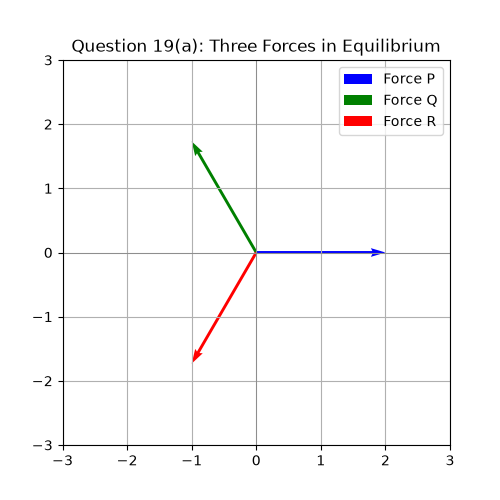
\includegraphics[width=0.6\textwidth]{figs/q19_fig}
			\caption{Three forces in static equilibrium.}
			\label{fig:q19_fig}
			\vspace{0.5em}
			\noindent\fbox{\parbox{\dimexpr\textwidth-2\fboxsep-2\fboxrule}{\hspace{2em}\textbackslash codes\textbackslash q19.py}}
		\end{figure}
		\item Setting support $A$ at $\vec{r}_A = \myvec{0 \\ 0}$ along the bridge axis gives support $B$ at $\vec{r}_B = \myvec{12 \\ 0}$, the bridge centroid at $\vec{r}_W = \myvec{6 \\ 0}$, and the lorry at $\vec{r}_L = \myvec{\frac{2}{3}\brak{12} \\ 0} = \myvec{8 \\ 0}$. From \eqref{eq:static_equilibrium_forces}, vertical force balance $\sum \vec{F}_k = \vec{0}$ gives $R_A + R_B = 56000 + 33600 = 89600\text{ N}$, and rotational equilibrium $\sum \vec{r}_k^{\top}\vec{J}\vec{F}_k = 0$ about $\vec{r}_A$ gives:
		\begin{align}
			12 R_B = \brak{56000 \times 6} + \brak{33600 \times 8} \implies R_B = 50400\text{ N}, \quad R_A = 39200\text{ N}
		\end{align}
		\begin{figure}[H]
			\centering
			\includegraphics[width=0.65\textwidth]{figs/q19b_fig}
			\caption{Bridge load distribution and support reactions in coordinate space.}
			\label{fig:q19b_fig}
			\vspace{0.5em}
			\noindent\fbox{\parbox{\dimexpr\textwidth-2\fboxsep-2\fboxrule}{\hspace{2em}\textbackslash codes\textbackslash 19b.py}}
		\end{figure}
		\item Formulating the convex LPP in matrix form \eqref{eq:lpp_cvxpy_form} with $\vec{x} = \myvec{x \\ y} \succeq \vec{0}$ and $\vec{c} = \myvec{6 \\ 10}$:
		\begin{align}
			\min_{\vec{x}} \; \vec{c}^{\top}\vec{x} \quad \text{s.t.} \quad \myvec{1 & 2 \\ 2 & 2 \\ 3 & 1}\myvec{x \\ y} \succeq \myvec{10 \\ 12 \\ 8}
		\end{align}
		Solving via \texttt{cvxpy} and corner-point evaluation of the feasible region yields minimum cost $Z = \text{Rs. } 52$ at $\vec{x}^* = \myvec{2 \\ 4}$ ($x = 2\text{ kg}, y = 4\text{ kg}$).
		\begin{figure}[H]
			\centering
			\includegraphics[width=0.65\textwidth]{figs/q19c_fig}
			\caption{Feasible region and optimal diet solution via \texttt{cvxpy}.}
			\label{fig:q19c_fig}
			\vspace{0.5em}
			\noindent\fbox{\parbox{\dimexpr\textwidth-2\fboxsep-2\fboxrule}{\hspace{2em}\textbackslash codes\textbackslash 19c.py}}
		\end{figure}
		\begin{figure}[H]
			\centering
			\noindent\fbox{\parbox{\dimexpr\textwidth-2\fboxsep-2\fboxrule}{\hspace{2em}\textbackslash codes\textbackslash 19c.c}}
		\end{figure}
		\item Formulating the convex LPP in matrix form \eqref{eq:lpp_cvxpy_form} (converting $6\text{ hrs} = 360\text{ min}$) with $\vec{x} = \myvec{x \\ y} \succeq \vec{0}$ and $\vec{c} = \myvec{0.75 \\ 0.50}$:
		\begin{align}
			\max_{\vec{x}} \; \vec{c}^{\top}\vec{x} \quad \text{s.t.} \quad \myvec{12 & 6 \\ 18 & 0 \\ 6 & 9}\myvec{x \\ y} \preceq \myvec{360 \\ 360 \\ 360}
		\end{align}
		Solving via \texttt{cvxpy} and feasible-polygon corner analysis yields maximum daily profit $Z = \text{Rs. } 26.25$ at $\vec{x}^* = \myvec{15 \\ 30}$ ($15$ cups of type A and $30$ cups of type B).
		\begin{figure}[H]
			\centering
			\includegraphics[width=0.65\textwidth]{figs/q19d_fig}
			\caption{Feasible region and optimal production mix via \texttt{cvxpy}.}
			\label{fig:q19d_fig}
			\vspace{0.5em}
			\noindent\fbox{\parbox{\dimexpr\textwidth-2\fboxsep-2\fboxrule}{\hspace{2em}\textbackslash codes\textbackslash 19d.py}}
		\end{figure}
		\begin{figure}[H]
			\centering
			\noindent\fbox{\parbox{\dimexpr\textwidth-2\fboxsep-2\fboxrule}{\hspace{2em}\textbackslash codes\textbackslash 19d.c}}
		\end{figure}
	\end{enumerate}
	
\end{enumerate}